%PROF:NAAM MOHAMED
%عالج باستخدام XeLaTeX
\documentclass[8pt,a4paper]{article}
\usepackage[left=1.2cm,right=1.2cm,top=1.6cm,bottom=2.2cm]{geometry}
\usepackage[x11names,usenames,dvipsnames,svgnames,table]{xcolor}
\usepackage{na-box}
\usepackage{yagusylo}
\usepackage{rotating}
\usepackage{url}
\usepackage{hyperref}
%\usepackage[pages=all]{background}
\hypersetup{pdfstartview=FitH,colorlinks=true, linkcolor=blue, urlcolor=red}
\usepackage{titlesec}
\usepackage{varwidth}
\usepackage[listings]{tcolorbox}
\usepackage{esvect}
\usepackage{tcolorbox, graphicx,  tikz}
\usepackage{graphicx}
\usepackage{tikz}
\usepackage[framemethod=tikz]{mdframed}
\usepackage[tikz]{bclogo}
\usepackage{pgf,tikz}  
\usepackage{calc,tikz}
\usepackage{contour}
\usetikzlibrary[shadings]
\usetikzlibrary{decorations.footprints}
\usetikzlibrary{shadows}
\usetikzlibrary{shapes.symbols}
\usetikzlibrary{shapes.symbols}
\tcbuselibrary{listings,breakable}
\usetikzlibrary{shapes.callouts}
\usetikzlibrary{decorations.pathmorphing}
\usetikzlibrary{patterns}
\usetikzlibrary{shapes,shadings,shadows,shapes.geometric,decorations,positioning,arrows,decorations.pathmorphing}
\usetikzlibrary{calc,fadings,shapes.geometric,shapes.misc, decorations.pathmorphing,shadows}
 \tcbuselibrary{skins,breakable}
\usetikzlibrary{calc}
\tcbuselibrary{listings}
\usetikzlibrary{decorations.pathmorphing}
\usepackage{tkz-tab}
\usepackage{array,tabularx}
\usepackage{fancybox}
\usepackage{multido}
\usepackage{etex}
\usepackage{amsmath,amsfonts,amssymb,mathrsfs} 
\usepackage{fourier}
\tcbuselibrary{listings,breakable,skins}
\usepackage{esvect}
\usepackage{fancyhdr}
\usepackage{ulem}  
\usepackage{tikz}
\usepackage{listings}
%\backgroundsetup{
	%scale=1,
	%opacity=1.0,
%	angle=0,
	%color=black,
	%contents={%
		%\ifodd\value{page}
			%\includegraphics[width=\paperwidth]{sss}
			%\else
			%\includegraphics[width=\paperwidth]{sss}
		%\fi
		%}
	%}
\tikzset{caixa/.style=
	{draw=green, top color=pink, bottom  color=white,shading angle=45,%rounded corners=5pt, inner xsep=5pt, inner ysep=6pt, outer ysep=10pt,drop shadow
	}
}
\tikzset{mdfshadow/.style={drop shadow=}}%

%%%this works well
\mdfdefinestyle{caixa}{userdefinedwidth=0.98\textwidth,%
	font=\small,%
	shadow=true,%
	shadowsize=5pt,%
	roundcorner=5pt,%
	align=center,%
	%leftmargin=0.3\textwidth,%
	%rightmargin=0.3\textwidth,%
	linecolor=green,%
	innerleftmargin=4pt,%
	innerrightmargin=4pt,
	apptotikzsetting
	={\tikzset{mdfbackground/.append style=caixa} }}
\tcbuselibrary{listings,breakable,skins}
\lstset{
    language=[LaTeX]TeX,escapeinside={*}{*},
  texcsstyle=*\color{red!40!black},
basicstyle=\ttfamily,
numbers=none,
	frame=none,
	rulesepcolor=\color{blue},
	rulecolor=\color{blue},
	framexleftmargin=10pt ,
breaklines=true,
keywordstyle=\color{blue},
commentstyle=\color{gray},
moretexcs={setdefaultlanguage,newfontfamily
, AtBeginDocument,arabicfon,lyfont},
morekeywords={begin, end, draw,fill,tcbuselibrary,
filldraw,shadedraw,shade,usetikzlibrary,foreach,clip,plot ,grid,rectangle,cycle,circle,path,pgfmathsetmacro
,radiusSmall},}
\usepackage{polyglossia}
\makeatletter 
\AtBeginDocument{\bidi@isloaded[]{arabxetex}}
\makeatother
\setdefaultlanguage[calendar=gregorian,locale=algeria]{arabic}
\newfontfamily\arabicfont[Script=Arabic,Scale=1.4]{Amiri}
\newfontfamily\arabicfontsf[Script=Arabic,Scale=1.4]{Amiri}
\newfontfamily
\bantiii[Script=Arabic,Scale=1.6]{Arial}
\newfontfamily
\bantii[Script=Arabic,Scale=1]{Arial}
\newfontfamily
\bantia[Script=Arabic,Scale=1.2]{Arial}
\newfontfamily\arabicfonttt[Scale=1]{Latin Modern Mono}
\newfontfamily\arabicfontttt[Scale=2]{Latin Modern Mono}
\newfontfamily
\dfont[Script=Arabic,Scale=1.5]{Amiri}
\setotherlanguage{french}
\usepackage[novoc]{arabxetex}
\DeclareGraphicsRule{.mps}{eps}{*}{}   
\newenvironment{NA}{%
\begin{bclogo}[logo = \bccrayon ,couleur=Gold,couleurBarre = red!50!black, arrondi = 0, ombre = false]{ \color{green!50!black}{\textarabic{ ملاحظة هامة  }}}%
}
{%
\end{bclogo}
}  
\newenvironment{NAA}{%
\begin{bclogo}[logo = \bcattention ,couleur=CadetBlue1,couleurBarre = red!30!black, arrondi = 0.1, ombre = true]{ \color{magenta}{\textarabic{تنبيه}}}%
}
{%
\end{bclogo}
}  
\newtcblisting{myboxx}{
	enhanced,
	frame style={	
			left color=blue,
			right color=blue},
	boxrule=0.7pt,
	colback=blue,
	breakable,
	listing options={escapeinside={*}{*},
		 texcsstyle=*\color{red!40!black},
basicstyle=\setLTR\ttfamily,
numbers=none,
	frame=none,
	rulesepcolor=\color{blue},
	rulecolor=\color{blue},
	framexleftmargin=10pt ,
breaklines=true,
keywordstyle=\color{blue},
commentstyle=\color{gray},
moretexcs={setdefaultlanguage,newfontfamily
, AtBeginDocument,arabicfon,lyfont},
morekeywords={begin, end, draw,fill,tcbuselibrary,
filldraw,shadedraw,shade,usetikzlibrary,foreach,clip,plot ,grid,rectangle,cycle,circle,path,pgfmathsetmacro
,radiusSmall},
		numberstyle=\tiny\color{red!75!black}},
	interior style={
		draw=blue!50!black,
		top color=yellow!15,
		bottom color=white},
	  segmentation style={
		draw=blue!50!black,
		solid,
		decorate,
		decoration={random steps,segment length=3mm}
}} 

\newtcblisting{mybox}{
enhanced,
colback=SpringGreen!20,
colframe=red!50!black,breakable,
bicolor,colbacklower=white,
listing options={language={[LaTeX]TeX},escapeinside={*}{*},
texcsstyle=*\color{red!50!black},
basicstyle=\setLTR\arabicfonttt,
numbers=none,
breaklines=true,
keywordstyle=\color{blue},
commentstyle=\color{gray},
moretexcs={},
morekeywords={begin, end, draw,fill,tcbuselibrary,
filldraw,shadedraw,shade,usetikzlibrary,foreach,clip,plot ,grid,rectangle,cycle,circle,path,pgfmathsetmacro
,radiusSmall}, % you can add what you need  
frame=none,
}}
\newtcblisting{boxn}{
enhanced,
 text side listing,
colback=SpringGreen,
colframe=red!50!black,breakable,
bicolor,colbacklower=white,
listing options={language={[LaTeX]TeX},escapeinside={*}{*},
texcsstyle=*\color{red!50!black},
basicstyle=\setLTR\arabicfonttt,
numbers=none,
breaklines=true,
keywordstyle=\color{blue},
commentstyle=\color{gray},
moretexcs={},
morekeywords={begin, end, draw,fill,tcbuselibrary,
filldraw,shadedraw,shade,usetikzlibrary,foreach,clip,plot ,grid,rectangle,cycle,circle,path,pgfmathsetmacro
,radiusSmall}, % you can add what you need  
frame=none,
}}
\newtcblisting{boxlis}{
enhanced,
colback=Aqua!60,
colframe=red!50!black,breakable,
listing only,
listing options={language={[LaTeX]TeX},escapeinside={*}{*},
texcsstyle=*\color{red!50!black},
basicstyle=\setLTR\arabicfonttt,
numbers=none,
breaklines=true,
keywordstyle=\color{blue},
commentstyle=\color{gray},
moretexcs={setdefaultlanguage,setdefaultlanguage,newfontfamily
,textarabic,hfill,uline,bf,breakbox,env,XeLaTeX,textfrench,underline,ztotpages,cfoot,rfoot,lfoot,chead,lhead,rhead, AtBeginDocument,arabicfon,usetikzlibrary,setotherlanguage,lyfont,arabicfontsf,arabicfont},
morekeywords={begin,end,draw,fill}, % you can add what you need  
frame=none,
}}
\definecolor{section@title@color}{cmyk}{1,0.2,0.3,0.1}
\definecolor{subsection@title@color}{cmyk}{0,0.6,0.9,0}
\definecolor{shadow@color}{cmyk}{.07,0,0,0.49}
\definecolor{lawn}{rgb}{0.49,0.95,0.85}
\definecolor{box}{rgb}{0.72,1.00,1.00}
\definecolor{bclogo}{rgb}{0.73,0.00,0.73}
\definecolor{d}{rgb}{0.73,1.00,0.73}
\definecolor{hyp}{rgb}{0.00,0.00,0.59}
\definecolor{sec}{rgb}{0.44,0.00,0.22}
% fontes section
\def\sectiontitle@font{\dfont \selectfont}
\def\subsectiontitle@font{\dfont \selectfont}
\newlength\decalnumsec
\newlength\decalnumsubsec
\setlength{\decalnumsec}{-0.5em}
\setlength{\decalnumsubsec}{-0.5em}
\newlength\decalxtitlesubsec
\setlength{\decalxtitlesubsec}{\parindent}
% Espace entre le numéro de section et le titre
\newlength\spacetitlesec
\newlength\spacetitlesubsec
\setlength{\spacetitlesec}{0.2em}
\setlength{\spacetitlesubsec}{0.2em}
\titleformat{\section}[block]
{%
	\bfseries\Large
	\color{sec}
	\sectiontitle@font
}
{
\raisebox{\decalnumsec}
{%
\begin{tikzpicture}
\node (numsec) {\sectiontitle@font\thesection};
\node [top color=SpringGreen, shading angle=45,star,drop shadow] at  (numsec) {\bantiii\thesection};
\end{tikzpicture}
}
}
{\spacetitlesec}
{}
\titleformat{\subsection}[block]
{%
	\bfseries
	\color{magenta!80!black}
	\subsectiontitle@font
}
{
\raisebox{\decalnumsubsec}
{%
\begin{tikzpicture}
\node (numsubsec) { \subsectiontitle@font\RL{\thesubsection}};
\node [top color=blue!50!white, shading angle=90,ellipse,drop shadow] at  (numsec) {\bantiii \RL{\thesubsection}};
\end{tikzpicture}
}
}
{\spacetitlesubsec}
{}
\definecolor{monstertandark}{HTML}{F0DBB5}	
\newcommand*{\E}{\ensuremath{\mathrm{e}}}
%Peach!20
\colorlet{codebackground}{LightBlue!30!white}
\renewcommand{\footrulewidth}{0pt}
\renewcommand{\headrulewidth}{0pt}
\renewcommand{\baselinestretch}{1.4}
%\tcbset{arc,arc is angular} 
\newcommand{\naams}[1]{\fcolorbox{brown}{brown}{{\color{white}\textbf{#1}}}}
\newtcolorbox{molahadaT}[1][]{enhanced,breakable,
  before skip=2mm,after skip=3mm,
  boxrule=0.4pt,left=5mm,right=0.7cm,top=1mm,bottom=1mm,
   interior style image=lazz.png,
  colframe=blue!50!black,
  sharp corners,rounded corners=southwest,arc is angular,arc=3mm,
  underlay={%
    \path[fill=tcbcol@back!80!black] ([yshift=3mm]interior.south west)--++(+0.4,+0.1)--++(-0.1,-0.4);
    \path[draw=tcbcol@frame,shorten <=-0.05mm,shorten >=-0.05mm] ([yshift=3mm]interior.south west)--++(+0.4,+0.1)--++(-0.1,-0.4);
    },
  drop fuzzy shadow,#1}
\newtcolorbox{paperbox}[2][]{
	frame hidden,
	boxrule=0pt,
	breakable,
	enhanced,
	before skip=11pt plus 1pt,
	toptitle=3mm,
	boxsep=0.25ex,
	left=8pt,
	right=8pt,
	fonttitle= \Large \waalidfontta \selectfont\scshape\bfseries\color{blue!50!black},
	fontupper=\sffamily \selectfont,
	title=#2,
	arc=0mm,
	parbox = false,
	borderline north={1pt}{-0.5pt}{black},
	borderline south={1pt}{-0.5pt}{black},
	interior style image=goldshade.png,
	colframe=monstertandark,
	title style image=goldshade.png,
	fuzzy shadow={0mm}{-3.5pt}{-0.5pt}{0.4mm}{black!60!white},
	overlay={
		\fill [fill=black] (frame.south west) -- ++(7pt,0) -- ++(0,-5pt) -- cycle;
		\fill [fill=black] (frame.north west) -- ++(7pt,0) -- ++(0,5pt) -- cycle;
		\fill [fill=black] (frame.north east) -- ++(-7pt,0) -- ++(0,5pt) -- cycle;
		\fill [fill=black] (frame.south east) -- ++(-7pt,0) -- ++(0,-5pt) -- cycle;
		},
	after={\vspace{10pt plus 1pt}\noindent},
	#1
}  
\makeatletter
\newtcolorbox{algeriabox}[2][]{%
enhanced,
breakable,
colback=white,
colframe=blue!30!black,
attach boxed title to top right={yshift=-2pt}, title={#2},
boxrule=0pt,
boxed title style={%
    sharp corners, 
    rounded corners=northeast, 
    colback=tcbcol@frame, 
    boxrule=0pt},
sharp corners=north,
overlay unbroken={%
    \path[fill=tcbcol@back] 
        ([xshift=2pt]title.south west) 
        to[out=180, in=0] ([xshift=-1.5cm]title.west)--
        (title.west-|frame.west) |- 
        ([xshift=2pt]title.south west)--cycle;
    \path[fill=tcbcol@frame] (title.south west) 
        to[out=180, in=0] ([xshift=-1.5cm]title.west)--
        (title.west-|frame.west)
        [rounded corners=\kvtcb@arc] |- 
        (title.north-|frame.north) 
        [sharp corners] -| (title.south west);
    \draw[line width=.5mm, rounded corners=\kvtcb@arc, 
        tcbcol@frame] 
        (title.north east) rectangle 
        (frame.south west);
}, 
overlay first={%
    \path[fill=tcbcol@back] 
        ([xshift=2pt]title.south west) 
        to[out=180, in=0] ([xshift=-1.5cm]title.west)--
        (title.west-|frame.west) |- 
        ([xshift=2pt]title.south west)--cycle;
    \path[fill=tcbcol@frame] (title.south west) 
        to[out=180, in=0] ([xshift=-1.5cm]title.west)--
        (title.west-|frame.west)
        [rounded corners=\kvtcb@arc] |- 
        (title.north-|frame.north) 
        [sharp corners] -| (title.south west);
    \draw[line width=.5mm, rounded corners=\kvtcb@arc, 
        tcbcol@frame] 
        (frame.south west) |- (title.north) -| 
        (frame.south east);
}, 
overlay middle={%
    \draw[line width=.5mm, tcbcol@frame] 
    (frame.north west)--(frame.south west) 
    (frame.north east)--(frame.south east);
}, 
overlay last={%
    \draw[line width=.5mm, rounded corners=\kvtcb@arc, 
        tcbcol@frame] 
        (frame.north west) |- (frame.south) -|
        (frame.north east);
}, 
#1
}
\newtcolorbox{naas}[2][]{%
enhanced,
breakable,
colback=white,
colframe=blue!30!black,
attach boxed title to top right={yshift=-2pt}, title={#2},
boxrule=0pt,
boxed title style={%
    sharp corners, 
    rounded corners=northeast, 
    colback=tcbcol@frame, 
    boxrule=0pt},
sharp corners=north,
overlay unbroken={%
    \path[fill=tcbcol@back] 
        ([xshift=2pt]title.south west) 
        to[out=180, in=0] ([xshift=-1.5cm]title.west)--
        (title.west-|frame.west) |- 
        ([xshift=2pt]title.south west)--cycle;
    \path[fill=tcbcol@frame] (title.south west) 
        to[out=180, in=0] ([xshift=-1.5cm]title.west)--
        (title.west-|frame.west)
        [rounded corners=\kvtcb@arc] |- 
        (title.north-|frame.north) 
        [sharp corners] -| (title.south west);
    \draw[line width=.5mm, rounded corners=\kvtcb@arc, 
        tcbcol@frame] 
        (title.north east) rectangle 
        (frame.south west);
}, 
overlay first={%
    \path[fill=tcbcol@back] 
        ([xshift=2pt]title.south west) 
        to[out=180, in=0] ([xshift=-1.5cm]title.west)--
        (title.west-|frame.west) |- 
        ([xshift=2pt]title.south west)--cycle;
    \path[fill=tcbcol@frame] (title.south west) 
        to[out=180, in=0] ([xshift=-1.5cm]title.west)--
        (title.west-|frame.west)
        [rounded corners=\kvtcb@arc] |- 
        (title.north-|frame.north) 
        [sharp corners] -| (title.south west);
    \draw[line width=.5mm, rounded corners=\kvtcb@arc, 
        tcbcol@frame] 
        (frame.south west) |- (title.north) -| 
        (frame.south east);
}, 
overlay middle={%
    \draw[line width=.5mm, tcbcol@frame] 
    (frame.north west)--(frame.south west) 
    (frame.north east)--(frame.south east);
}, 
overlay last={%
    \draw[line width=.5mm, rounded corners=\kvtcb@arc, 
        tcbcol@frame] 
        (frame.north west) |- (frame.south) -|
        (frame.north east);
}, 
#1
}
\definecolor{myblue}{RGB}{40,96,139}
\definecolor{fondpaille}{cmyk}{0,0,0.1,0}
\makeatother
\parindent=0pt
%\pagecolor{brown!10}
\tcbset{arc=2mm}
\makeatletter%
\renewcommand\tableofcontents%
{%
  %\section*{\contentsname}%
  \@mkboth{%
  \MakeUppercase\contentsname}{\MakeUppercase\contentsname}%
  \@starttoc{toc}%
}
\rightfootnoterule
\newcommand{\widecheckperso}[1]{%
3 \overset{\rotatebox{180}{$\widehat{\hphantom{#1}}$}}{#1}}
\newcommand{\colorUL}[1][black]
{%
\bgroup%
\ifdim\ULdepth=\maxdimen
  \settodepth\ULdepth{(j}%
  \advance\ULdepth.4pt
\fi
\markoverwith{\kern0em\vtop{%
\kern\ULdepth {%
\color{#1}\hrule   width .4em}}%
\kern0em}\ULon}

\newcommand{\colorULdotted}[1][black]
{%
\bgroup%
\ifdim\ULdepth=\maxdimen
  \settodepth\ULdepth{(j}%
  \advance\ULdepth.4pt
\fi
\markoverwith{\kern0em\vtop{%
\kern\ULdepth {%
\color{#1}\hrule width .6em}}
\kern0em}\ULon}
\newenvironment{reflet}[1]
{
\begin{center}
\begin{tikzpicture}[inner sep=3pt]
\node[scale=1.4,above,yslant=0]{#1};
\node[scale=1.4,above,yslant=0,
yscale=-1,scope fading=south,
opacity=0.4]{#1};
\end{tikzpicture}
}
{
\end{center}}
 \def\mosqdoor{%
{15}% Horizontal center
{0}b{15}\\% Text begins at x=15, y=0
{1}t{13}{4}\\%
{2}t{10.5}{9}\\%
{3}t{8.5}{13}\\%
{4}t{7.2}{15.6}\\%
{5}t{6.3}{17.4}\\%
{6}t{5.5}{19}\\%
{7}t{4.8}{20.4}\\%
{8}t{4.3}{21.4}\\%
{9}t{4.1}{21.8}\\%
{9.5}t{3.9}{22.2}\\%
{10}t{4.1}{21.8}\\%
{11}t{4.3}{21.4}\\%
{12}t{4.5}{21}\\%
{13}t{5}{20}\\%
{14}t{5.8}{18.4}\\%
{15}t{7}{16}\\%
{17}t{7}{16}\\%
{18}t{7}{16}\\% <<
{18.1}t{6}{18}\\%
{19}t{6}{18}\\%
{20}t{5}{20}\\%
{29}t{5}{20}\\%
{30}e{15}%
}
\newcommand{\bola}{\tikz \node [shading angle=45,shading=ball , ball color=yellow,semicircle,drop shadow] at (0,0) { \bantii \thepage};}
\newcommand{\etoile}[1]{\tikz \node [ shading angle=45,top color=CadetBlue1,star,star points=6,drop shadow] at (0,0) { #1};}
\newcommand{\mos}[1]{\tikz \node [ shading angle=45,shading=ball , ball color=LightSlateBlue ,rectangle,rounded corners=5pt,drop shadow] at (0,0) { #1};}
\newcommand{\nono}[1]{\tikz \node [ shading angle=45,shading=ball , ball color=Aquamarine1 ,starburst,drop shadow] at (0,0) { #1};}
\newcommand{\nona}[1]{\tikz\node [shading=ball , ball color=Aquamarine1,draw,thick, minimum height=1cm, minimum width=3cm,
      decorate, decoration={random steps,segment length=3pt,amplitude=1pt}]
      {#1};}
    
\newcommand{\draalg}{\begin{tikzpicture}[scale=0.8]
  % Use wikipedia's dimensions
  \filldraw[fill=white](0,0) rectangle (12, 8);
  \fill[fill=ForestGreen,draw=black](0,0) rectangle (6, 8);
  \draw(9,7)node[right]{\small \textarabic{تحيا الجزائر}};
  \fill[red] (6,4) circle (1.5);
  \begin{scope}
  \clip (0,0) rectangle (6,8);
  \fill[ForestGreen] (6.4,4) circle (1.2);
  \end{scope}
  \begin{scope}
  \clip (6,0) rectangle (12,8);
  \fill[white] (6.4,4) circle (1.2);
  \end{scope}
  \node[star,fill=red, minimum size=1.4cm, rotate=-18, star point ratio=2.617,inner sep=0pt,xshift=1.5mm] at (6.4,4) {};
  % Star point ratio is GoldenRatio^2 (1.618^2)
\end{tikzpicture}}



\begin{document}
\title{\etoile{ \LARGE \textarabic{الحزمة
\texttt{na-box}}}\\
\vspace*{-4\baselineskip}
\textfrench{Version 1.0}
\vspace*{3\baselineskip}
}

\author{\mos{\tikz{
 \draw (0,0) node {\resizebox {15cm}{1cm}{\contour{black}{ \color{white}{\textarabic{ \yagding[ark]{117} لرسم إطارات ملونة لكتابة دروس في الرياضيات }}}}}}}\\
\textarabic{  تم إنشاء هذه الحزمة إعتمادا على تعديل  في الحزمة
\texttt{pas-cours} 
}}
\date{
\nono{ \color{red}\textarabic{ \small   من تعديل الأستاذ : ناعم محمد
}}}

\maketitle

\vspace{-1cm}
\hrulefill
\thispagestyle{empty}
\begin{center}
\draalg
\end{center}

\pagestyle{empty}
\newpage
\pagestyle{fancy}
\cfoot{\bola}
\lhead{}
\rhead{ }  
\lfoot{}
\onecolumn
\setcounter{page}{1}
\pagenumbering{arabic}


\begin{mdframed}[style=caixa]
 \begin{arab}
lqd qmt b-'in^sA' al.hzmT \texttt{na-box} 
w hy .hzmT thtmm brsm 'i.tArAt mlwwnT lktAbT t`Aryf , mlA.h.zAt , brAhyn , xwA.s ,...-'ilx . \\
w h_dh al.hzmT 'an^s-'at 'i`tmAdA `lY
t`dyl fy  al.hzmT \texttt{pas-cours} \\
al.hzmT \texttt{na-box} ymkn 'istxdAmhA `nd alm`AljT b--- \texttt{XeLaTeX} w `nd 'istxdAm al.hzmT \texttt{polyglossia}\\ 
tAb`wnA fy alfysbwk `lY 
\colorbox{yellow}{\textarabic{مجموعة الأستاذ ناعم محمد}} 
'aw `lY  \href{http://www.facebook.com/groups/latex.fans/}{ \textarabic{ مجموعة محبي } \textfrench{\LaTeX}}.
\end{arab}
\end{mdframed}
\begin{arab}
\section{ كيفية تثبيت الحزمة على  \textfrench{TeX Live}  } 
\underline {\underline { الخطوة الاولى :}}  
al.hzmT \colorbox{yellow}{\texttt{na-box}} `bArT `n mjlld y.htwy mlf mn 'imtdAd \texttt{sty} , lt_tybthA `lY altAk lAyf , qm bnsx almjlld  \texttt{na-box} al_dy y.hwy almlf \texttt{na-box.sty} w .d`h wfq almsAr alttAly :
\LR{ \verb# C:\texlive\texmf-local\tex\latex\local #} , w al.swwrT alttAlyyT tw.d.h mrA.hl  _dlk 
\begin{center}
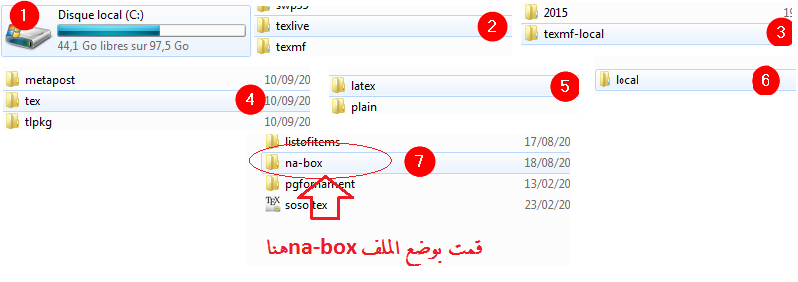
\includegraphics[height=5cm,width=18cm]{nabox}
\end{center}
\underline {\underline { الخطوة الثانية :}} 
nqwm bft.h \LR{\texttt{TeX Live Manager}}
w nanf_d al`mlytyn almbyntyn fy al.swwr 'adnAh 
\begin{center}
 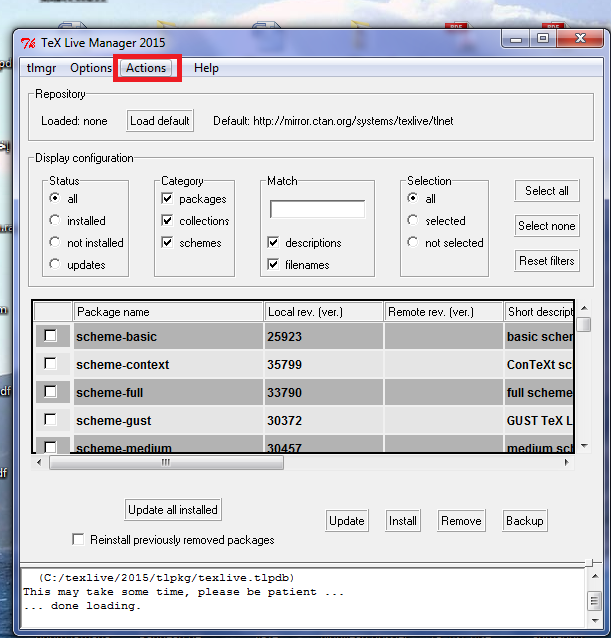
\includegraphics[height=10cm,width=12cm]{29}
\end{center}
\begin{center}
 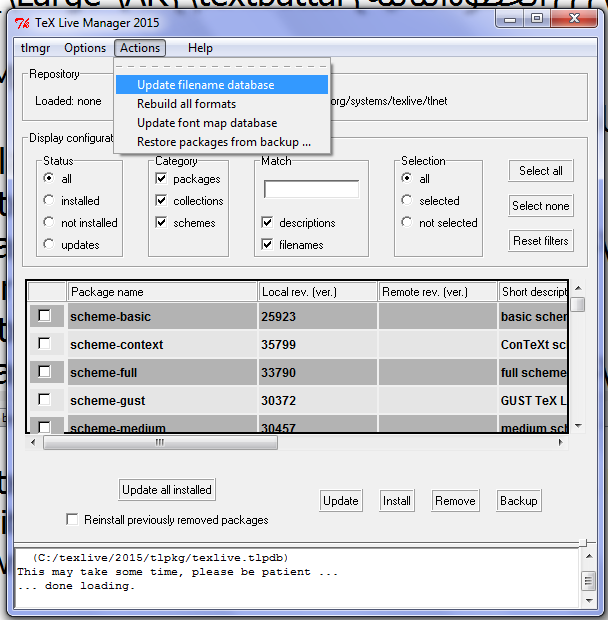
\includegraphics[height=10cm,width=12cm]{30}
\end{center}
\begin{center}
 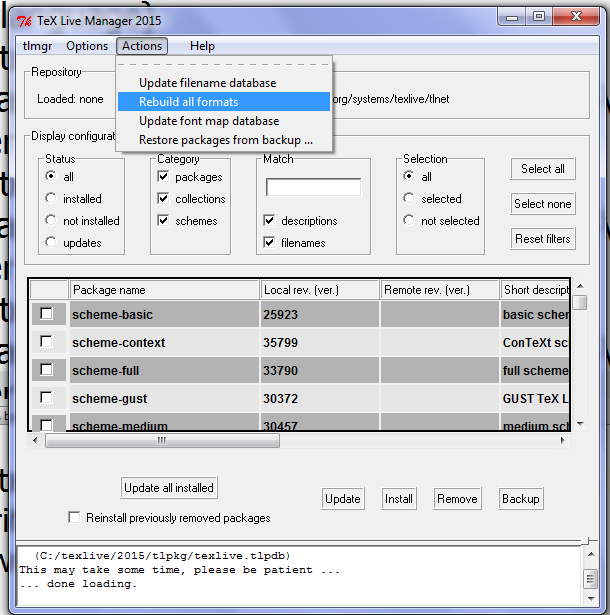
\includegraphics[height=10cm,width=12cm]{31}
\end{center}
bh_dh al.tryqT tkwn qd qmt bt_tbyt h_dh al.hzmT `lY \textfrench{TeX Live} w l-'ist`mAlhA mA `lyk 'ilA 'an tktb m` al.hzm  mA yly : \LR{ \verb# \usepackage{na-box} #}
\begin{NA}
ymkn t_tbyt al.hzmT alssAbqT `lY{\bf \textfrench{TeX Live}} b.trq 'axrY , w ymknk 'an tst`mhA dwn t_tbythA  w fy h_dh al.hAlT lAbd 'an tnsx almlf \texttt{na-box.sty} w t.d`h dA'imA fy almjlld al_dy t`Alj fyh , b.tby`T al.hAl b`d 'an tktb m` al.hzm  
\LR{ \verb# \usepackage{na-box} #} 
\end{NA}
\section{ كيفية إستخدام الحزمة و رسم الإطارات } 
al.hzmT 'an^s-'at x.sy.sA lrsm 'i.tArAt mlwwnT lktAbT t`Aryf , mlA.h.zAt ; xwA.s ; brAhyn ; ntA'ij ,m_tAl , tmAryn, 'an^s.tT, .trA'iq .....-'ilx . \\ ymkn al-'i`tmAd `lyhA lktAbT drws fy alrryA.dyAt  bAstxdAm l.gT
alttAk m` al.hzmT  \LR{ \verb# \usepackage{polyglossia} #}
\subsection{التعليمة \textfrench{$\setminus$env}  و رسم الإطارات  }
ymkn rsm mxtlf al-'i.tArAt bAstxdAm altt`lymT
\LR{ \verb#\env[style=?]{....} #}
.hy_t 'amAm klmT \texttt{style} w fy mkAn `lAmT al-'istfhAm nktb nw` al-'i.tAr w hy kmA yly : \\
\yagding[ifsymgeonarrow]{82}
\texttt{xwas} lktAbT xA.syyT \\
\yagding[ifsymgeonarrow]{82}
\texttt{borhan} lktAbT albrhAn \\
\yagding[ifsymgeonarrow]{82}
\texttt{molahadt} lktAbT mlA.h.zT \\
\yagding[ifsymgeonarrow]{82}
\texttt{ta3ryf} lktAbT t`ryf \\
\yagding[ifsymgeonarrow]{82}
\texttt{mbarhanat} lktAbT mbrhnT\\
\yagding[ifsymgeonarrow]{82}
\texttt{ntyjt} lktAbT ntyjT\\
\yagding[ifsymgeonarrow]{82}
\texttt{mital} lktAbT m_tAl \\
\yagding[ifsymgeonarrow]{82}
\texttt{nachat} lktAbT n^sA.t \\
\yagding[ifsymgeonarrow]{82}
\texttt{tryqt} lktAbT .tryqT \\
mkAn alnnq.t alty byn .hA.dntyn nkbt n.s almbrhnT , altt`ryf, alxA.syyT, alm_tAl , ....-'ilx. nstxdm alal.gT al`rbyT  `n .tryq lw.hT almfAty.h w nktb b^skl `Ady .
\subsection*{أمثلة}
\subsection*{مثال أول}
\begin{boxlis}
\env[style=ta3ryf]
{*\textarabic{\bantii
نسمي متتالية حسابية ، كل متتالية عددية   }*
$(U_n)$
*\textarabic{\bantii
تحقق ما يلي : }*
$U_{n+1}=U_n+r$
*\textarabic{\bantii
حيث}*
$r$
*\textarabic{\bantii
عدد حقيقي ثابت ، يسمى أساس المتتالية الحسابية }*
$(U_n)$
}
\end{boxlis}
nt.h.s.sl b`d alm`AljT b-- \texttt{XeLaTeX}
`lY al-'i.tAr alttAly:
\end{arab}
\env[style=ta3ryf]
{نسمي متتالية حسابية 
، كل متتالية 
$(U_n)$
تحقق ما يلي :
$U_{n+1}=U_n+r$
حيث 
$r$
عدد حقيقي ثابت ، يسمى أساس المتتالية الحسابية 
$(U_n)$
}
\subsection*{مثال ثاني}
\begin{arab}
\begin{boxlis}
\env[style=xwas]
{*\textarabic{\bantii
نسمي متتالية حسابية ، كل متتالية عددية   }*
$(U_n)$
*\textarabic{\bantii
تحقق ما يلي : }*
$U_{n+1}=U_n+r$
*\textarabic{\bantii
حيث}*
$r$
*\textarabic{\bantii
عدد حقيقي ثابت ، يسمى أساس المتتالية الحسابية }*
$(U_n)$
}
\end{boxlis}
nt.h.s.sl b`d alm`AljT b-- \texttt{XeLaTeX}
`lY al-'i.tAr alttAly:
\end{arab}
\env[style=xwas]
{نسمي متتالية حسابية 
، كل متتالية 
$(U_n)$
تحقق ما يلي :
$U_{n+1}=U_n+r$
حيث 
$r$
عدد حقيقي ثابت ، يسمى أساس المتتالية الحسابية 
$(U_n)$
}
\subsection*{مثال ثالث}
\begin{arab}
\begin{boxlis}
\env[style=mbarhanat]
{*\textarabic{\bantii
نسمي متتالية حسابية ، كل متتالية عددية   }*
$(U_n)$
*\textarabic{\bantii
تحقق ما يلي : }*
$U_{n+1}=U_n+r$
*\textarabic{\bantii
حيث}*
$r$
*\textarabic{\bantii
عدد حقيقي ثابت ، يسمى أساس المتتالية الحسابية }*
$(U_n)$
}
\end{boxlis}
nt.h.s.sl b`d alm`AljT b-- \texttt{XeLaTeX}
`lY al-'i.tAr alttAly:
\end{arab}
\env[style=mbarhanat]
{نسمي متتالية حسابية 
، كل متتالية 
$(U_n)$
تحقق ما يلي :
$U_{n+1}=U_n+r$
حيث 
$r$
عدد حقيقي ثابت ، يسمى أساس المتتالية الحسابية 
$(U_n)$
}
\subsection*{مثال رابع}
\begin{arab}
\begin{boxlis}
\env[style=borhan]
{*\textarabic{\bantii
نسمي متتالية حسابية ، كل متتالية عددية   }*
$(U_n)$
*\textarabic{\bantii
تحقق ما يلي : }*
$U_{n+1}=U_n+r$
*\textarabic{\bantii
حيث}*
$r$
*\textarabic{\bantii
عدد حقيقي ثابت ، يسمى أساس المتتالية الحسابية }*
$(U_n)$
}
\end{boxlis}
nt.h.s.sl b`d alm`AljT b-- \texttt{XeLaTeX}
`lY al-'i.tAr alttAly:
\end{arab}
\env[style=borhan]
{نسمي متتالية حسابية 
، كل متتالية 
$(U_n)$
تحقق ما يلي :
$U_{n+1}=U_n+r$
حيث 
$r$
عدد حقيقي ثابت ، يسمى أساس المتتالية الحسابية 
$(U_n)$
}
\subsection*{مثال خامس}
\begin{arab}
\begin{boxlis}
\env[style=ntyjt]
{*\textarabic{\bantii
نسمي متتالية حسابية ، كل متتالية عددية   }*
$(U_n)$
*\textarabic{\bantii
تحقق ما يلي : }*
$U_{n+1}=U_n+r$
*\textarabic{\bantii
حيث}*
$r$
*\textarabic{\bantii
عدد حقيقي ثابت ، يسمى أساس المتتالية الحسابية }*
$(U_n)$
}
\end{boxlis}
nt.h.s.sl b`d alm`AljT b-- \texttt{XeLaTeX}
`lY al-'i.tAr alttAly:
\end{arab}
\env[style=ntyjt]
{نسمي متتالية حسابية 
، كل متتالية 
$(U_n)$
تحقق ما يلي :
$U_{n+1}=U_n+r$
حيث 
$r$
عدد حقيقي ثابت ، يسمى أساس المتتالية الحسابية 
$(U_n)$
}
\subsection*{مثال سادس}
\begin{arab}
\begin{boxlis}
\env[style=molahadt]
{*\textarabic{\bantii
نسمي متتالية حسابية ، كل متتالية عددية   }*
$(U_n)$
*\textarabic{\bantii
تحقق ما يلي : }*
$U_{n+1}=U_n+r$
*\textarabic{\bantii
حيث}*
$r$
*\textarabic{\bantii
عدد حقيقي ثابت ، يسمى أساس المتتالية الحسابية }*
$(U_n)$
}
\end{boxlis}
nt.h.s.sl b`d alm`AljT b-- \texttt{XeLaTeX}
`lY al-'i.tAr alttAly:
\end{arab}
\env[style=molahadt]
{نسمي متتالية حسابية 
، كل متتالية 
$(U_n)$
تحقق ما يلي :
$U_{n+1}=U_n+r$
حيث 
$r$
عدد حقيقي ثابت ، يسمى أساس المتتالية الحسابية 
$(U_n)$
}
\begin{arab}
\subsection{خواص إضافية في التعليمة \textfrench{$\setminus$env} }
ymkn 'i.dAfT xwA.s fy altt`lymT \LR{ \verb# \env #} tw.d` dAxl almxlbyn w hy :\\
\LR{ \verb# [pluriel,degrade,name={\textarabic{.....}},notitle] #}\\
\yagding[ifsymgeowide]{3}
\texttt{pluriel} lky t-'aty `nAwyn al-'i.tArAt alssAbqT `lY ^skl mjmw` m_tlA  lw nktb 
\LR{ \verb#\env[style=ta3ryf,pluriel]{....} #} 
sy-'aty al-'i.tAr b`nwAn t`Aryf 'ay jm` t`ryf\\
\yagding[ifsymgeowide]{3}
\texttt{degrade} lky y-'aty lwn al-'i.tAr mtdrj\\
\yagding[ifsymgeowide]{3}
\LR{ \verb#name={\textarabic{.....}} #}
lktAbT `nwAn fr`y lil-'i.tAr y-'aty fy 'aq.sY alysAr.\\
\yagding[ifsymgeowide]{3}
\LR{ \verb#notitle #}
lrsm 'i.tAr dwn `nwAn
\subsection*{أمثلة}
\end{arab}
\subsection*{مثال أول}
\begin{arab}
\begin{boxlis}
\env[style=ta3ryf,pluriel]
{*\textarabic{\bantii
نسمي متتالية حسابية ، كل متتالية عددية   }*
$(U_n)$
*\textarabic{\bantii
تحقق ما يلي : }*
$U_{n+1}=U_n+r$
*\textarabic{\bantii
حيث}*
$r$
*\textarabic{\bantii
عدد حقيقي ثابت ، يسمى أساس المتتالية الحسابية }*
$(U_n)$
}
\end{boxlis}
nt.h.s.sl b`d alm`AljT b-- \texttt{XeLaTeX}
`lY al-'i.tAr alttAly:
\end{arab}
\env[style=ta3ryf,pluriel]
{نسمي متتالية حسابية 
، كل متتالية 
$(U_n)$
تحقق ما يلي :
$U_{n+1}=U_n+r$
حيث 
$r$
عدد حقيقي ثابت ، يسمى أساس المتتالية الحسابية 
$(U_n)$
}
\subsection*{مثال ثاني}
\begin{arab}
\begin{boxlis}
\env[style=mbarhanat,name=\textarabic{*\textarabic{\bantii
تقبل دون برهان }*}]
{*\textarabic{\bantii
نسمي متتالية حسابية ، كل متتالية عددية   }*
$(U_n)$
*\textarabic{\bantii
تحقق ما يلي : }*
$U_{n+1}=U_n+r$
*\textarabic{\bantii
حيث}*
$r$
*\textarabic{\bantii
عدد حقيقي ثابت ، يسمى أساس المتتالية الحسابية }*
$(U_n)$
}
\end{boxlis}
nt.h.s.sl b`d alm`AljT b-- \texttt{XeLaTeX}
`lY al-'i.tAr alttAly:
\end{arab}
\env[style=mbarhanat,name=\textarabic{تقبل دون برهان}]
{نسمي متتالية حسابية 
، كل متتالية 
$(U_n)$
تحقق ما يلي :
$U_{n+1}=U_n+r$
حيث 
$r$
عدد حقيقي ثابت ، يسمى أساس المتتالية الحسابية 
$(U_n)$
}
\subsection*{مثال ثالث}
\begin{arab}
\begin{boxlis}
\env[style=mbarhanat,degrade,name=\textarabic{*\textarabic{\bantii
تقبل دون برهان }*}]
{*\textarabic{\bantii
نسمي متتالية حسابية ، كل متتالية عددية   }*
$(U_n)$
*\textarabic{\bantii
تحقق ما يلي : }*
$U_{n+1}=U_n+r$
*\textarabic{\bantii
حيث}*
$r$
*\textarabic{\bantii
عدد حقيقي ثابت ، يسمى أساس المتتالية الحسابية }*
$(U_n)$
}
\end{boxlis}
nt.h.s.sl b`d alm`AljT b-- \texttt{XeLaTeX}
`lY al-'i.tAr alttAly:
\end{arab}
\env[style=mbarhanat,degrade,name=\textarabic{تقبل دون برهان}]
{نسمي متتالية حسابية 
، كل متتالية 
$(U_n)$
تحقق ما يلي :
$U_{n+1}=U_n+r$
حيث 
$r$
عدد حقيقي ثابت ، يسمى أساس المتتالية الحسابية 
$(U_n)$
}
\subsection*{مثال رابع}
\begin{arab}
\begin{boxlis}
\env[style=mbarhanat,notitle]
{*\textarabic{\bantii
نسمي متتالية حسابية ، كل متتالية عددية   }*
$(U_n)$
*\textarabic{\bantii
تحقق ما يلي : }*
$U_{n+1}=U_n+r$
*\textarabic{\bantii
حيث}*
$r$
*\textarabic{\bantii
عدد حقيقي ثابت ، يسمى أساس المتتالية الحسابية }*
$(U_n)$
}
\end{boxlis}
nt.h.s.sl b`d alm`AljT b-- \texttt{XeLaTeX}
`lY al-'i.tAr alttAly:
\end{arab}
\env[style=mbarhanat,notitle]
{نسمي متتالية حسابية 
، كل متتالية 
$(U_n)$
تحقق ما يلي :
$U_{n+1}=U_n+r$
حيث 
$r$
عدد حقيقي ثابت ، يسمى أساس المتتالية الحسابية 
$(U_n)$
}
%\itemclass{black}
\subsection{الوسط \textfrench{nabox} }
\begin{arab}
alws.t \textfrench{nabox} ysm.h 'ay.dA brsm al-'i.tArAt alssAbqT b^skl `Ady , alws.t ^sklh al`Am kmA yly :
\begin{boxlis}
\begin{nabox}[style=?,pluriel,degrade,name={\textarabic{...}},notitle]
*\textarabic{\bantii
المحتوى }*
\end{nabox}
\end{boxlis}
\begin{NAA}
fymA yx.s alxwA.s almwjwdT byn mxlbyn ymkn alt.hkkm fyhA kmA fy altt`lymT 
\LR{ \verb# \env #}
\end{NAA}
\end{arab}
\subsection*{أمثلة}
\subsection*{مثال أول}
\begin{arab}
\begin{boxlis}
\begin{nabox}[style=mital]
*\textarabic{\bantii
نسمي متتالية حسابية ، كل متتالية عددية   }*
$(U_n)$
*\textarabic{\bantii
تحقق ما يلي : }*
$U_{n+1}=U_n+r$
*\textarabic{\bantii
حيث}*
$r$
*\textarabic{\bantii
عدد حقيقي ثابت ، يسمى أساس المتتالية الحسابية }*
$(U_n)$
\end{nabox}
\end{boxlis}
nt.h.s.sl b`d alm`AljT b-- \texttt{XeLaTeX}
`lY al-'i.tAr alttAly:
\end{arab}
\begin{nabox}[style=mital]
نسمي متتالية حسابية 
، كل متتالية 
$(U_n)$
تحقق ما يلي :
$U_{n+1}=U_n+r$
حيث 
$r$
عدد حقيقي ثابت ، يسمى أساس المتتالية الحسابية 
$(U_n)$
\end{nabox}
\subsection*{مثال ثاني}
\begin{arab}
\begin{boxlis}
\begin{nabox}[style=tamryn]
*\textarabic{\bantii
أكتب هنا نص التمرين.............................
..................   }*

\end{nabox}
\end{boxlis}
nt.h.s.sl b`d alm`AljT b-- \texttt{XeLaTeX}
`lY al-'i.tAr alttAly:
\end{arab}
\begin{nabox}[style=tamryn]
أكتب هنا نص التمرين.............................
..................
\end{nabox}
\subsection*{مثال ثالث}
\begin{arab}
\begin{boxlis}
\begin{nabox}[style=nachat]
*\textarabic{\bantii
أكتب هنا نص النشاط.............................
..................   }*

\end{nabox}
\end{boxlis}
nt.h.s.sl b`d alm`AljT b-- \texttt{XeLaTeX}
`lY al-'i.tAr alttAly:
\end{arab}
\begin{nabox}[style=nachat]
أكتب هنا نص النشاط.............................
..................
\end{nabox}
\subsection*{مثال رابع}
\begin{arab}
\begin{boxlis}
\begin{nabox}[style=tryqt,pluriel,name={\textarabic{*\textarabic{\bantii
حساب إتجاه تغير متتاليية }*}}]
*\textarabic{\bantii
أكتب هنا نص الطرائق.............................
..................   }*

\end{nabox}
\end{boxlis}
nt.h.s.sl b`d alm`AljT b-- \texttt{XeLaTeX}
`lY al-'i.tAr alttAly:
\end{arab}
\begin{nabox}[style=tryqt,pluriel,name={\textarabic{
حساب إتجاه تغير متتاليية }}]
أكتب هنا نص الطرائق.............................
..................
\end{nabox}
\subsection{التعليمة  \textfrench{$\setminus$breakbox}}
\begin{arab}
tsA`d altt`lymT  \LR{ \verb# \breakbox #}
fy alws.t \LR{ \verb# nabox #}
`lY rsm 'i.tArAt lhA fA.sl , b`nY 'Axr fy b`.d al.hAlAt ykwn alm.htwY .twylA mamA yj`l al-'i.tAr yntql 'ilY al.sf.hT almwAlyyT , ltfAdy wqw` _dlk , nstxdm altt`lymT  \LR{ \verb# \breakbox #} fy alws.t \LR{ \verb# nabox #}
\end{arab}
\subsection*{أمثلة}
\subsection*{مثال أول}
\begin{arab}
\begin{boxlis}
\begin{nabox}[style=tamryn]
*\textarabic{\bantii
نص التمرين   }*
.......................
........................
\breakbox
*\textarabic{\bantii
إكمال نص التمرين  }*
\end{nabox}
\end{boxlis}
nt.h.s.sl b`d alm`AljT b-- \texttt{XeLaTeX}
`lY al-'i.tAr alttAly:
\end{arab}
\begin{nabox}[style=tamryn]
نص التمرين
.......................
........................
\breakbox
إكمال نص التمرين
\end{nabox}
\subsection*{مثال ثاني}
\begin{arab}
\begin{boxlis}
\begin{nabox}[style=tamryn,notitlebreak]
*\textarabic{\bantii
نص التمرين   }*
.......................
........................
\breakbox
*\textarabic{\bantii
إكمال نص التمرين  }*
\end{nabox}
\end{boxlis}
nt.h.s.sl b`d alm`AljT b-- \texttt{XeLaTeX}
`lY al-'i.tAr alttAly:
\end{arab}
\begin{nabox}[style=tamryn,notitlebreak]
نص التمرين
.......................
........................
\breakbox
إكمال نص التمرين
\end{nabox}
\begin{arab}
altt`lymT \LR{ \verb# notitlebreak #}
alty 'a.dfthA byn mxlbyn , tsm.h b-'il.gA'  `nwAn al-'i.tAr `nd alfA.sl , kmA fy alm_tAl alssAbq 
\subsection{الترقيم مع الحزمة \textfrench{na-box}}
tsm.h al.hzmT \textfrench{na-box}
bw.d` al-'arqAm dAxl 'i.tArAt .s.gyrT mlwwnT fy alws.t \textfrench{enumerate} , w 'ay.dA tsm.h bAlttlwyn fy alws.t 
\textfrench{itemize}
\end{arab}
\subsection*{أمثلة}
\subsection*{مثال أول}
\begin{arab}
\begin{boxlis}
\itemclass{black}
\begin{enumerate}
\item *\textarabic{\bantii
نص عربي }*
\item *\textarabic{\bantii
نص عربي }*
\end{enumerate}
\end{boxlis}
nt.h.s.sl b`d alm`AljT b-- \texttt{XeLaTeX}
`lY al-'i.tAr alttAly:
\end{arab}
\itemclass{black}
\begin{enumerate}
\item 
نص عربي 
\item 
نص عربي
\end{enumerate}
أضفت هنا التعليمة 
\LR{ \verb# \itemclass{black} #}
لجعل لون إطارات الارقام هو اللون الأسود ، يمكنك ان تغير اللون كما تشاء
\subsection*{مثال ثاني}
\begin{arab}
\begin{boxlis}
\itemclass{black}
\begin{enumerate}
\item *\textarabic{\bantii
نص عربي }*
\item *\textarabic{\bantii
نص عربي }*
\end{enumerate}
\itemclass{green}
\begin{enumerate}
\item *\textarabic{\bantii
نص عربي }*
\item *\textarabic{\bantii
نص عربي }*
\end{enumerate}
\end{boxlis}
nt.h.s.sl b`d alm`AljT b-- \texttt{XeLaTeX}
`lY al-'i.tAr alttAly:
\end{arab}
\itemclass{black}
\begin{enumerate}
\item 
نص عربي 
\item 
نص عربي
\end{enumerate}
\itemclass{green}
\begin{enumerate}
\item 
نص عربي 
\item 
نص عربي 
\end{enumerate}
\subsection*{مثال ثالث}
\begin{arab}
\begin{boxlis}
\itemclass{black}
\begin{enumerate}
\item *\textarabic{\bantii
نص عربي }*
\item *\textarabic{\bantii
نص عربي }*
\begin{itemize}
\item *\textarabic{\bantii
نص عربي }*
\item *\textarabic{\bantii
نص عربي }*
\end{itemize}
\end{enumerate}
\itemclass{red}
\begin{enumerate}
\item *\textarabic{\bantii
نص عربي }*
\item *\textarabic{\bantii
نص عربي }*
\begin{itemize}
\item *\textarabic{\bantii
نص عربي }*
\item *\textarabic{\bantii
نص عربي }*
\end{itemize}
\end{enumerate}
\end{boxlis}
nt.h.s.sl b`d alm`AljT b-- \texttt{XeLaTeX}
`lY al-'i.tAr alttAly:
\end{arab}
\itemclass{black}
\begin{enumerate}
\item 
نص عربي 
\item 
نص عربي
\begin{itemize}
\item 
نص عربي
\item 
نص عربي 
\end{itemize}
\end{enumerate}
\itemclass{red}
\begin{enumerate}
\item 
نص عربي 
\item 
نص عربي 
\begin{itemize}
\item 
نص عربي
\item 
نص عربي 
\end{itemize}
\end{enumerate}
\subsection*{مثال رابع}
\begin{arab}
\begin{boxlis}
\begin{nabox}[style=tamryn]
*\textarabic{\bantii
نص التمرين   }*
.......................
........................
\itemclass{black}
\begin{enumerate}
\item *\textarabic{\bantii
نص عربي }*
\item *\textarabic{\bantii
نص عربي }*
\begin{itemize}
\item *\textarabic{\bantii
نص عربي }*
\end{itemize}
\end{enumerate}
\breakbox
*\textarabic{\bantii
إكمال نص التمرين  }*
\itemclass{red}
\begin{enumerate}
\item *\textarabic{\bantii
نص عربي }*
\item *\textarabic{\bantii
نص عربي }*
\begin{itemize}
\item *\textarabic{\bantii
نص عربي }*
\item *\textarabic{\bantii
نص عربي }*
\end{itemize}
\end{enumerate}
\end{nabox}
\end{boxlis}
nt.h.s.sl b`d alm`AljT b-- \texttt{XeLaTeX}
`lY al-'i.tAr alttAly:
\end{arab}
\begin{nabox}[style=tamryn]
نص التمرين 
.......................
........................
\itemclass{black}
\begin{enumerate}
\item 
نص عربي 
\item 
نص عربي 
\begin{itemize}
\item 
نص عربي 
\end{itemize}
\end{enumerate}
\breakbox
إكمال نص التمرين 
\itemclass{red}
\begin{enumerate}
\item 
نص عربي 
\item 
نص عربي 
\begin{itemize}
\item 
نص عربي 
\item 
نص عربي 
\end{itemize}
\end{enumerate}
\end{nabox}
\vspace{5cm}
\begin{reflet}{ \textarabic{تقبلوا تحيات الأستاذ ، الفقير إلى الله  : ناعم محمد}}
\end{reflet}
للإستفسار اكثر ، البريد الإلكتروني هو
\colorbox{lime}{\url{sosonaam13@hotmail.com}}
\end{document}

